\documentclass[12pt]{article}
\usepackage{amsmath,amsfonts,nicefrac}
\usepackage{graphicx}
\usepackage{enumerate}
\usepackage{natbib}
\usepackage{url} % not crucial - just used below for the URL 
\usepackage{ifthen}

%\pdfminorversion=4
% NOTE: To produce blinded version, replace "0" with "1" below.
\newcommand{\blind}{1}
% DON'T change margins - should be 1 inch all around.
\addtolength{\oddsidemargin}{-.5in}%
\addtolength{\evensidemargin}{-.5in}%
\addtolength{\textwidth}{1in}%
\addtolength{\textheight}{-.3in}%
\addtolength{\topmargin}{-.8in}%


\usepackage[table]{xcolor}% http://ctan.org/pkg/xcolor

\newcommand{\cl}[2]{\cellcolor{#1!#2}}
\newcommand{\inc}[2]{ \ifthenelse{\equal{#1}{1}}{\input{./sections/#2}}{ } }



\begin{document}

%\bibliographystyle{natbib}

\def\spacingset#1{\renewcommand{\baselinestretch}%
{#1}\small\normalsize} \spacingset{1}


%%%%%%%%%%%%%%%%%%%%%%%%%%%%%%%%%%%%%%%%%%%%%%%%%%%%%%%%%%%%%%%%%%%%%%%%%%%%%%

\if1\blind
{
  \title{\bf Towards Structured Use of Bayesian Sequential Monitoring in Clinical Trials}
  \author{Evan Kwiatkowski\textsuperscript{$\dagger$}, 
	        Eugenio Andraca-Carrera\textsuperscript{$\ddagger$},\\
					Mat Soukup\textsuperscript{$\ddagger$},
					\medskip Matthew A. Psioda\textsuperscript{$\dagger$}\thanks{The authors gratefully acknowledge \textit{please remember to list all relevant funding sources in the unblinded version}}\\
	  %
	  $\dagger$ Department of Biostatistics,
		University of North Carolina, \\
		McGavran-Greenberg Hall, CB\#7420, \\
		%
		\medskip Chapel Hill, North Carolina, U.S.A.\\
    $\ddagger$ Division of Biometrics VII, Office of Biostatistics \\
		           Center for Drug Evaluation and Research, \\
							 US Food and Drug Administration, \\
							 Silver Spring, Maryland, USA \\									
		}
  \maketitle
} \fi

\if0\blind
{
  \bigskip
  \bigskip
  \bigskip
  \begin{center}
    {\LARGE\bf Title}
\end{center}
  \medskip
} \fi

\bigskip
\begin{abstract}
The text of your abstract. 200 or fewer words.
\end{abstract}

\noindent%
{\it Keywords:}  3 to 6 keywords, that do not appear in the title
\vfill

\newpage
\spacingset{1.5} % DON'T change the spacing!



\section{Introduction}

Things to discuss:
\begin{itemize}
 \item 21\textsuperscript{st} Century Cures Act (MATT)
 \item PDUFA VI reauthorization (MATT)
 \item Expansive work already done on sequential monitoring  (EVAN -- draft on 6/21)
\begin{enumerate}
%\item Berry A Case for Bayesianism, Cornfield The Bayesian outlook, classical arguments for Bayes in clinical trials, not sequential monitoring in particular
%\item (1) Berry Montoring Accumulating Data, (2) Cornfield/Greenhouse On certain aspects, (3) Cornfield Sequential Trials, (4) A Bayesian Test of Some Classical Hypotheses, with Applications to Sequential Clinical Trials Jerome Cornfield 
%\item Bayes \& monitoring, based on posterior distributions
\item Foundational Bayesian sequential monitoring \cite{Cornfield1966}~\cite{Cornfield1966a}~\cite{Neyman1967}.
\item Further development \cite{Freedman1989}~\cite{Freedman1992}~\cite{Spiegelhalter1993}~\cite{Spiegelhalter1994}~\cite{Fayers1997}.
\item Need to go further, and mention work on 3-arm Bayesian trials.
%\item First papers in Bayes sequential monitoring. Bayesian inferences not affected by frequent or continual monitoring by the likelihood principle.
%\item Papers which compare to frequentist stopping rules \& increased interpretation on role of priors.
%\item \cite{Spiegelhalter1994}
%\item \cite{Spiegelhalter1993} predictive distributions as basis for monitoring
%\item \cite{Freedman1992} choice of prior explained by showing its impact on percentiles of posterior distribution
%\item \cite{Freedman1989} The need to overcome this `\textbf{handicap}' prevents unduly early termination.
%\item \cite{Fayers1997} Choosing these two priors (skeptical, enthuastic) provides a useful \textbf{brake} against the premature termination of trials.
%\item Bayesian Adaptive Methods for Clinical Trials Berry, Carlin, Etc.
\end{enumerate}
 \item Our majors contribution (EVAN -- as early as possible in introduction without having the flow appear weird -- draft on 6/21)
 \item Outline for the remaining section of the paper (EVAN -- draft on 6/21)
\end{itemize}
\section{Methods}

As you introduce ideas that come from or extend other ideas in the literature, cite the relevant literature.

\subsection{Monitoring versus Estimation Priors (EVAN -- draft on 6/21)}

%\begin{itemize}
% \item Define generally in terms of $\boldsymbol\theta = \left( \gamma, \boldsymbol\psi  \right)$ where $\gamma$ is a parameter of interest
%       and $\boldsymbol\psi$ is a nuisance parameter (possible vector valued).
% \item Define \textit{Monitoring} Priors and \textit{Inference} Priors.
% \item Make connection between Inference priors and two-part mixture prior and BMA.
% \item Define \textit{Skeptical} and \textit{Enthusiastic} monitoring priors and how each would be used.
% \item I would have a generic graphic to illustrate the types of priors and the mixture.
% %\item Motivate in the context of a simple example (i.e., single parameter binary example).
%\end{itemize}

\subsubsection{Bayesian hypothesis testing based on posterior probabilities}

The Bayesian framework allows direct inference on a parameter of interest through specification of a model for the data generating mechanism and prior distributions for unknown quantities. Let $\mathbf{D}$ be a random variable representing the data collected in the trial with density $p(\mathbf{D}|\theta,\psi)$ where $\theta$ and $\psi$ are the unknown quantities. Let $\theta$ be the parameter of interest and $\psi$ be the unknown quantities that are not of primary importance (i.e. ``nuisance parameters"). Define the sample spaces for the unknown quantities as $\theta\in\Theta$ and $\psi\in\Psi$. Suppose the hypotheses under consideration are $H_0:\theta\in\Theta_{H_0}$ versus $H_1:\theta\in\Theta_{H_1}$, where $\Theta=\Theta_{H_0}\cup \Theta_{H_1}$ and $\Theta_{H_0}\cap \Theta_{H_1}=\emptyset$. These hypotheses are adjudicated based on posterior probabilities of $\theta$ by evaluating $P(\theta\in\Theta_{H_i}|\mathbf{D})=\int_{\Theta_{H_i}}p(\theta|\mathbf{D})d\theta$ for $i\in\{0,1\}$, where $p(\theta|\mathbf{D})=\int_{\Psi}p(\theta,\psi|\mathbf{D})d\psi$. Define $\delta$ as a threshold for \textit{a compelling level of evidence} as it relates to $\theta$. We say that an individual is ``all but convinced" that $H_i$ is true given the observed data if $P(\theta\in\Theta_i|\mathbf{D})\geq\delta$ $i\in\{1,2\}$. The quantity $1-\delta$ reflects \textit{residual uncertainty} of $H_i$ being true relative to the competing hypothesis. For example, an individual would be ``all but convinced" of the truth of the alternative hypothesis if $P(\theta\in\Theta_{H_1}|\mathbf{D})\geq\delta$.

The posterior distribution of $\theta$ depends on the choice of prior distribution $\pi(\theta,\psi)$, since $p(\theta,\psi|\mathbf{D})=p(\mathbf{D}|\theta,\psi)\pi(\theta,\psi)/p(\mathbf{D})$ by Bayes rule. The specification of the prior distribution depends on the research objective. An \textit{inference prior} is a prior that is used when the research objective is to make final analysis after data collection is complete. A \textit{monitoring prior} is a prior that is used when the research objective is monitor enrollment with an eye towards early termination.
%Possible simplifying functional relationships between $\theta$ and $\psi$ are conditional independence $\pi(\theta,\psi)=\pi(\theta|\psi)\pi(\psi)$ and independence $\pi(\theta,\psi)=\pi(\theta)\pi(\psi)$. An inference prior is often non-informative or objective in the sense that it does not show preference to $H_0$ or $H_1$. Decisions made using using a non-informative prior are often similar to those made in the frequentist setting. 

It has been said that `the purpose of a trial is to collect data that bring to conclusive consensus at termination opinions that had been diverse and indecisive at the outset' (Kass and Greenhouse (1989)). These opinions manifest as priors $\pi(\theta,\psi)$ for which their relation to $P(\theta\in\Theta_i|\pi(\theta,\psi))$ $i\in\{0,1\}$ is examined (note this quantity does not depend on the data $\mathbf{D}$ and therefore reflect a-priori opinion). A skeptical prior is an informative or subjective prior that gives substantial preference to $H_0$ such that it is ``all but convinced" that $H_0$ is true a-priori. This prior $\pi_{S}(\theta,\psi)\equiv\pi_{S}$ has the property that $P(\theta\in\Theta_0| \pi_{S})\geq\delta$ (equivalently $P(\theta\in\Theta_1| \pi_{S})<1-\delta$). For example, if $\delta=0.95$, then this choice of skeptical prior places 95\% prior probability that $\theta\in\Theta_0$. An enthuastic prior $\pi_{E}(\theta,\psi)\equiv\pi_{E}$ similarly gives preference to $H_1$ through the property that $P(\theta\in\Theta_1| \pi_{E})\geq\delta$ (equivalently $P(\theta\in\Theta_0| \pi_{E})<1-\delta$). For purposes of interpretation, a \textit{skeptical person} is someone whose a-priori opinions of $\theta$ are reflected through a skeptical prior and a \textit{enthuastic person} is someone whose a-priori opinions of $\theta$ are reflected through an ethuastic prior.

The use of monitoring based on changing the opinion of skeptical and enthuastic priors has been described as overcoming a handicap (\cite{Freedman1989}) and providing a brake (\cite{Fayers1997}) on the premature termination of trials, or constructing ``an adversary who will need to be disilusioned by the data to stop further experimentation" (\cite{Spiegelhalter1994}). Early termination of the trial is appriopriate if diverse prior opinions about $\theta$ would be in agreement given the interm data. It is then reasonable to stop data collection if, upon seeing the data, a \textit{skeptical person} changes their opinion to be ``all but convinced" that $H_1$ is true ($P(\theta\in\Theta_1|\mathbf{D}, \pi_{S})\geq\delta$), or an \textit{enthuastic person} becomes ``all but convinced" that $H_1$ is false ($P(\theta\in\Theta_0|\mathbf{D}, \pi_{E})\geq\delta$).

%Summarizing~\cite{Spiegelhalter1993} and others:  or that the benefit of treatment is not likely to be what was expected, the probability of \textit{eventually} proving that $H_1$ is true is sufficiently low, or the resources have been exhausted.  
%A standard Bayesian decision rule would reject $H_0$ when $P(\theta\in\Theta_{H_1}|D\geq 0.95)$ which will result in a Type I error rate of $0.05$ when the analysis prior is non-informative (a so-called reference or flat prior). The Bayes factor in favor of $H_0$ is defined as 
%\begin{align*}
%BF=\frac{p(D|H_0)}{p(D|H_1)}=\frac{\int_{\Theta_{H_0}}p(D|\theta,H_0)\pi(\theta|H_0)d\theta}{\int_{\Theta_{H_1}}p(D|\theta,H_0)\pi(\theta|H_1)d\theta}
%\end{align*}
%and let $p(\theta|D,\pi)$ denote the posterior distribution of $\theta$ given a particular prior distribution.


Final inference on $\theta$ is made once enrollment is stopped based on the monitoring priors or at the planned end of the trial. An inference prior is often non-informative or objective in the sense that it does not show preference to $H_0$ or $H_1$. This prior $\pi_{I}(\theta,\psi)\equiv\pi_{I}$ has the property that $P(\theta\in\Theta_0|\pi_I)\approx P(\theta\in\Theta_1|\pi_I)$. We propose use of a mixture prior constructed from the monitoring process as the inference prior:
\begin{align*}
\pi_{I}=\omega\times\pi_{S}+(1-\omega)\times\pi_E
\end{align*}
for $\omega\in[0,1]$. Choosing $\omega=1/2$ corresponds to an agnostic inference prior. Choosing $\omega$ based on posterior model probabilities of the null and alternative hypothesis yields $\omega=p(\mathbf{D}| \pi_{S})/(p(\mathbf{D}| \pi_{S})+p(\mathbf{D}| \pi_{E}))$. All relevant information about $\theta$ can be derived from its posterior distribution with an inference prior (e.g. posterior mean, credible intervals). Define $p(\mathbf{D}|\pi)=\int L (\theta|\mathbf{D})\pi(\theta)d\theta$ to be the marginal likelihood for the data given the prior $\pi$. The posterior mean using the inference prior will be a two-part mixture of the posterior means using the skeptical and enthuastic priors:
\begin{align*}
E(\theta|\mathbf{D},\pi_{I})=\omega\times E(\theta|\mathbf{D}, \pi_{S})+(1-\omega)\times E(\theta|\mathbf{D}, \pi_{E}).
\end{align*}

%\begin{align*}
%\pi_{Inference}=\frac{p(\mathbf{D}| \pi_{S}) \pi_{S}+p(\mathbf{D}| \pi_{E}) \pi_{E}}{p(\mathbf{D}| \pi_{S})+p(\mathbf{D}| \pi_{E})}
%\end{align*}
%\begin{align*}
%E(\theta|\mathbf{D},\pi_{Inference})=\omega\times E(\theta|\mathbf{D}, \pi_{S})+(1-\omega)\times E(\theta|\mathbf{D}, \pi_{E})
%\end{align*}
%Need to describe relation to Type I and Type II error.
\subsubsection{Default parameterization of monitoring priors for common designs}\label{monitoring_prior_specification}
Define prior distribution as $\pi(\theta|\lambda)$ where $\lambda$ is a vector of hyperparameters.

Skeptical prior might be centered around the clinical inferiority boundary.
Enthuastic prior might be centered around clinical superiority boundry.
Variance based on tail area considerations, or by matching the skeptical prior variance.

Reference prior attempts to express no particular opinion about the treatment's merit. 



\subsection{Futility Monitoring Using Probability of Success (EVAN -- draft on 6/21)}

\begin{itemize}
 \item Futility monitoring using POS is about stopping early when their is a high likelihood
       of a study being inconclusive at the end of the study.
 \item Since the final analysis uses the \textit{Inference} prior, POS should be based on the
       inference prior.
 \item Develop the framework for POS and show how it is a weighted average POS based on the skeptical
       and enthusiastic priors.
\end{itemize}
As an alternative strategy to futility analysis, one can monitor the probability of success (POS) for the trial. The probability of getting a convincing result at the end of the trail can be computed using the interm data. Let $p(\theta|D, \pi_{I})$ denote the posterior distribution for $\theta$ based on the inference prior $ \pi_{I}$ and the current data $D$. Let $\omega$ denote the POS which is given as follows:
\begin{align*}
\omega=E[1\{P(\theta\in\Theta_1|D_1,D, \pi_{I})\geq 1-\delta\}]
\end{align*}
where the expectation is taken with respect to the posterior predictive distribution $p(D_1)$ for future data $D_1$ (ongoing + subjects yet to enroll):
\begin{align*}
p(D_1)=\int p(D_1|\theta)\times \pi(\theta|D)d\theta.
\end{align*}
One may stop the enrollment if $\omega$ is sufficiently small (i.e., $\omega<0.05$).

Stochastic curtailment in frequentist setting.
\section{Examples -- (EVAN)}

\subsection{Single-Arm Oncology Proof-of-Activity Trial w/ Binary Endpoint}
For example, consider testing the hypothesis $H_0:\theta\leq\theta_0$ versus $H_1:\theta>\theta_0$ where $\theta$ is a treatment effect of interest. Suppose an effect $\theta_1>\theta_0$ is thought to be highly clinically relevant and plausible given what limited data is available. Consider a clinical trial with a single analysis and fixed sample size chosen that there is a high probability of proving $H_1$ when $\theta=\theta_1$. A standard Bayesian decision rule would reject $H_0$ when $P(\theta>\theta_0|D)\geq 0.95$ which will result in a type one error rate of $0.05$ (approximately) if $\theta=\theta_0$ when the analysis prior is non-informative (a so-called reference or flat prior).

\subsubsection*{Vemurafenib Trial (\cite{Hyman2015})}
``In this study, a response rate of 15\% at week
8 was considered to be low, a response rate of
45\% was considered to be high, and a response
rate of 35\% was considered to be low but still
desirable and indicative of efficacy. Assuming
response rates as specified in the hypothesis testing, a power of 80\% for a high response rate and
70\% for the low but still desirable response rate,
and a two-sided alpha level of 0.1, we calculated
that the number of patients required in each
cohort would be 7, 13, or 19, depending on the
results obtained."
\subsection{Parallel Two-Group Superiority Trial /w Continuous Binary Endpoint}

\subsection{Three-Arm, Placebo Controlled Non-Inferiority Trial w/ Continuous Endpoint}

\section{Discussion -- (MATT/EVAN)}

%\section{Example of Parallel Two-Group Design}
%
%In this section we consider a sequential monitoring approach in a parallel two-group setting using a binary response endpoint.
%
%We consider the case where the goal is prove superiority of an investigational product (IP) to a control 
%which could be a placebo.
%
%Let $\pi_0$ represent the response rate the control group and $\pi_1$ represent the response probability for the IP group.
%
%Here we wish to elicit pessimistic and enthusiastic priors consistent with the following:
% \begin{enumerate}
%  \item The control group response probability is expected to be approximately $0.20$ and investigators are relatively sure
%		    that the it will be between 0.5 and 0.35.
%				
%	\item The IP group response probability is likely to provide an improvement of approximately 0.20.
%\end{enumerate}
%
%In this setting pessimism or optimism is reflected in the induced prior on the difference in proportions $\pi_1 - \pi_0$.
%
%One easy way to specify such a prior in this case is to elicit a bivariate normal prior for $\pi_0$ and $\pi_1$ truncated to the unit square.  


%
%		\begin{figure}
%      \centering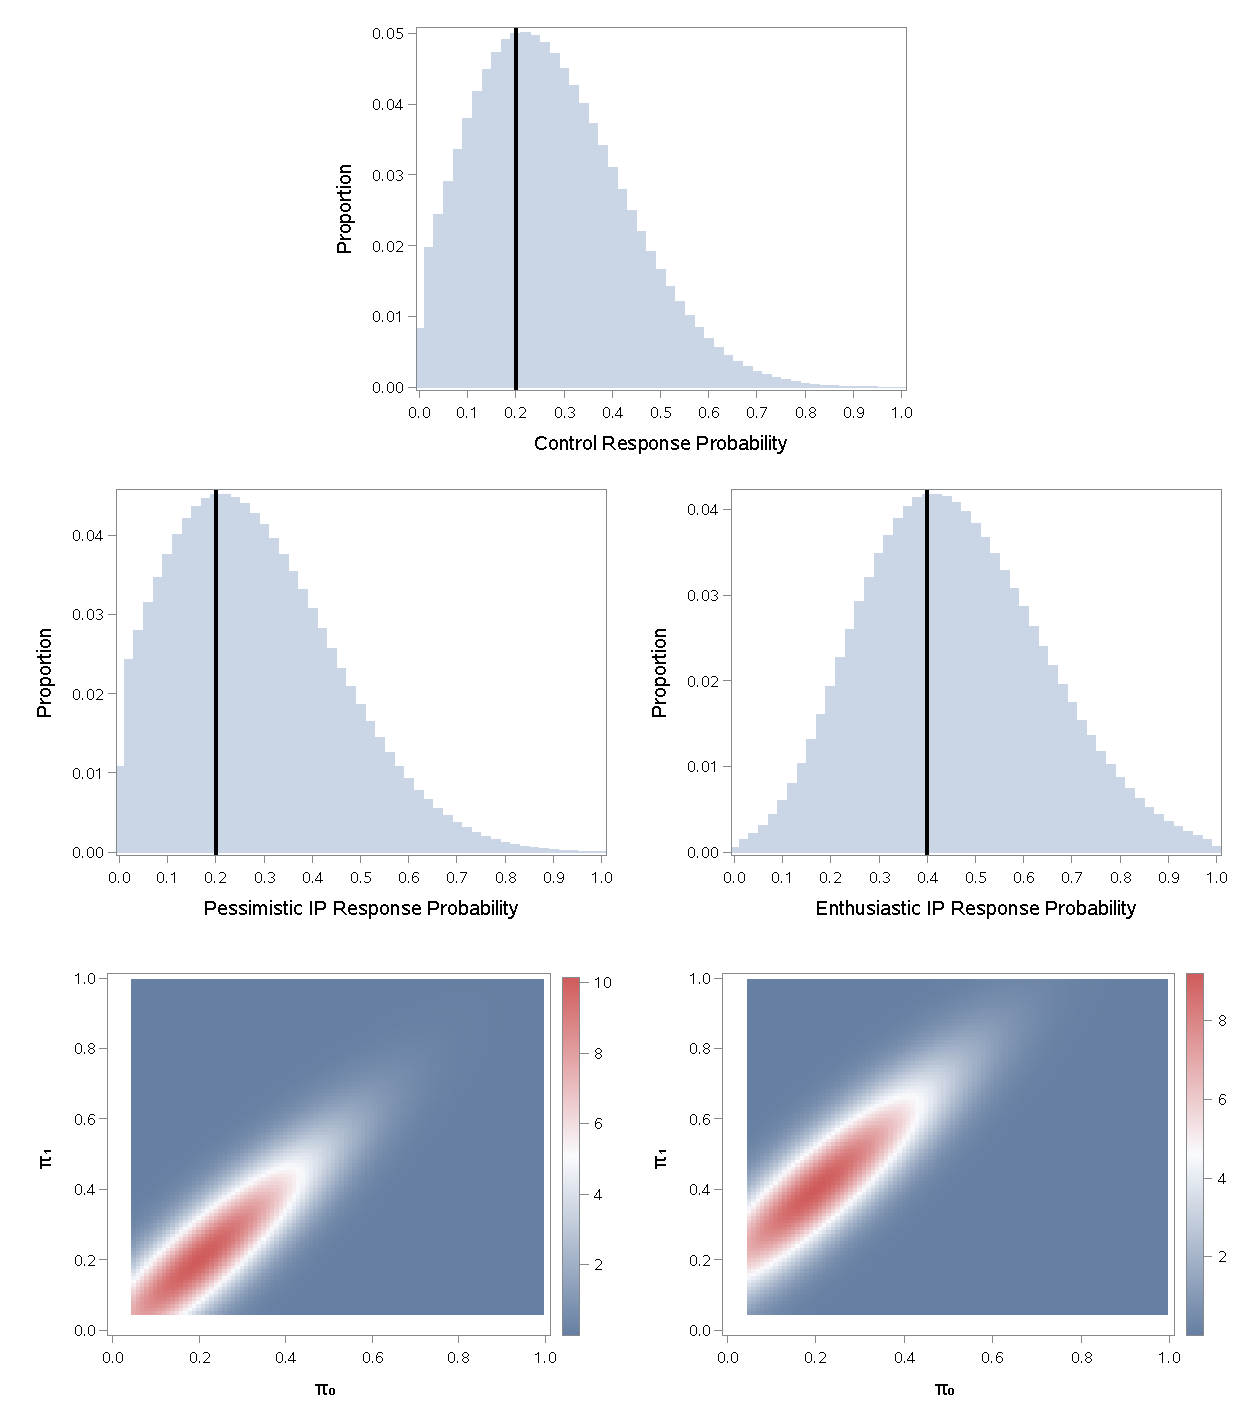
\includegraphics[scale=0.70]{./FIGURES/BINARY-PRIORS.pdf}
%      \caption{Prior for Control Group Response Probability \label{fig:pmp}}
%    \end{figure}
			
	

%\bigskip
\newpage
\begin{center}
{\large\bf SUPPLEMENTARY MATERIAL}
\end{center}


\section{BibTeX}

 \bibliographystyle{agsm}
 \bibliography{./References}		

\end{document}
